The CBGB apparatus design has various stages, a room temperature 300K outer aluminum vacuum chamber, onto which a Pulse Tube Refrigerator (PTR) is mounted, an aluminum radiation shield mounted to the 40K PTR cooling stage, and an inner copper cryopumping shield and experimental cell connected to the 4K PTR cooling stage. Connected to the vertical vacuum chamber, a "stem" region protrudes out from the beam side as seen in figures \cref{fig: SW chamber,fig: chamber} where a large turbo V551\todo{turbo deets} pumps down the entire volume. The beam comes out of the experimental cell and shield, through a set of apertures, into the stem region where skimmers and shutters are mounted to manipulate the beam.

A Cryomech PT415 PTR with a remote head option was attached to the top plate of the vacuum chamber with a large bellows mount to isolate the chamber from the mechanical vibrations caused by the PTR motor head. The chamber was pumped down to normal operating pressures, where then 4 retaining screws were tightened to just above the bellow's compressed height. This maintains mechanical decoupling between the outer vacuum chamber and the PTR while running.

We want to minimize the mechanically coupling onto the PTR due to the fragility of the pulse tube walls; small amounts of force applied onto a mechanically connected component would risk torquing the walls to break. Thus, all components inside the CBGB are mechanically connected to the top plate of the vacuum chamber via 8-32 stainless steel (SS316) threaded rods. Thermal connections are made with copper braids welded onto L-shaped brackets that mount between platforms secured to the PTR cooling stages and the shields.

Not only are all the inner shields connected to the top plate, but so are the feedthroughs including gas fill lines. This ensures that any and all connections made into the CBGB are not disturbed when opening the outer vacuum chamber to expose the inner components.

\begin{figure}[H]
	\centering
	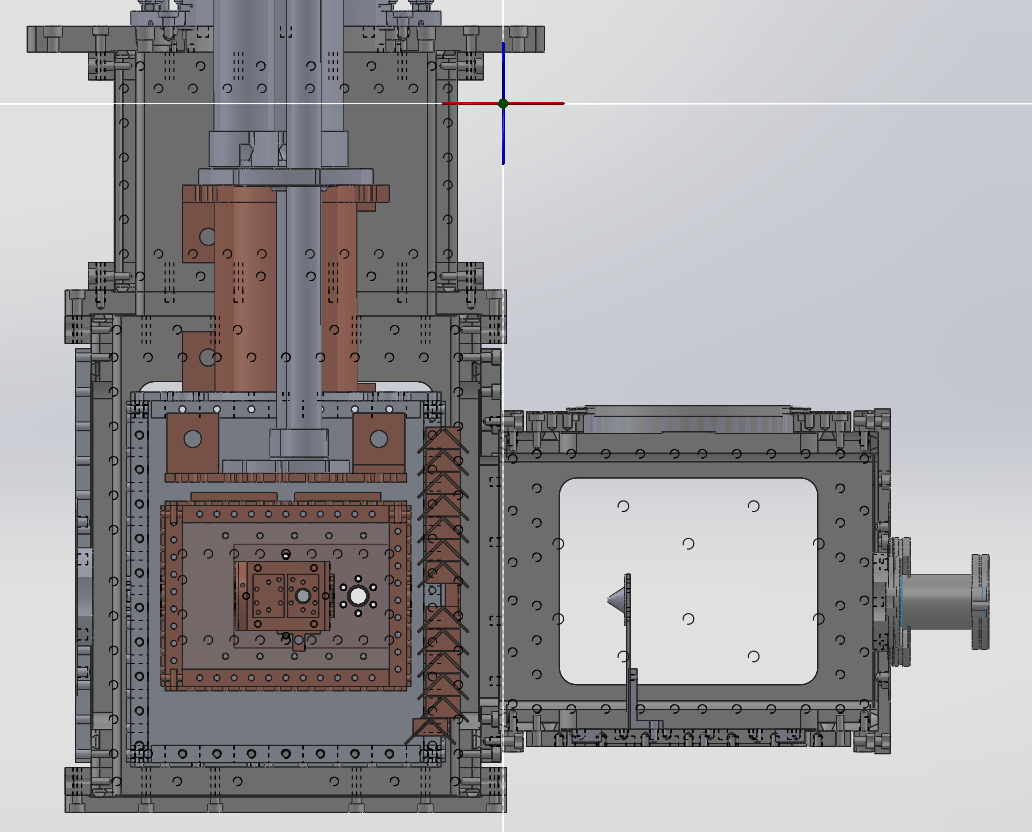
\includegraphics[width=1\textwidth]{images/CBGB_solidworks_cross_section.png}
	\caption{Cross sectional view of CBGB in solidworks. Components include copper sheath for PTR, aluminum radiation shield with chevron baffles, copper shield and experimental cell, and skimmer mounted in stem chamber. The baffles allow for gas to flow into the cold region of the beam apparatus, while preventing 300K black body radiation from hitting the inner shield and cell.}
	\label{fig: SW chamber}
\end{figure}

\begin{figure}[H]
	\centering
	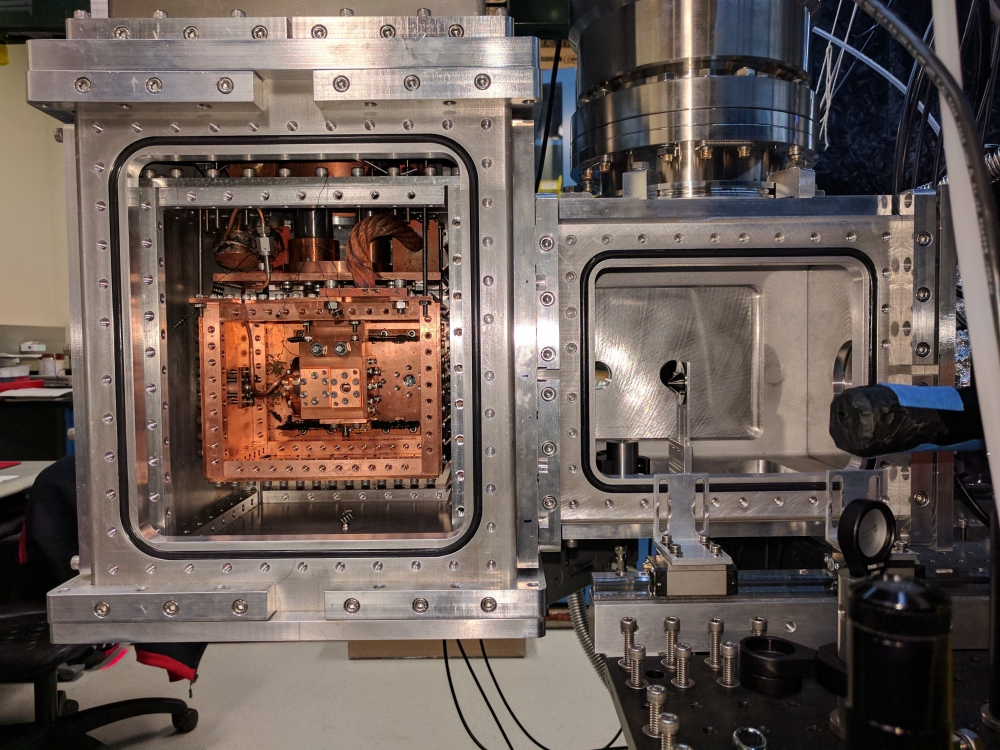
\includegraphics[width=1\textwidth]{images/CBGB_cross_section.jpg}
	\caption{Cross sectional view of CBGB with side walls removed from the outer vacuum chamber, 40K aluminum radiation shield, and inner 4K cryopumping shield exposing the inner experimental cell. A skimmer is mounted in the stem region.}
	\label{fig: chamber}
\end{figure}